% survey_0261002.pdf を川本先生の体裁で組み直したもの．
% コンパイル（slide/ で実行）:
%   lualatex -interaction=nonstopmode -output-directory=out survey_0261002.tex
\documentclass[aspectratio=169,10pt,t]{beamer}
\usepackage[ja]{labslide}

\graphicspath{{fig/survey/}}

\kicker{サーベイ}
\title{安全保障と好み選択を\\両立できる局所プランナ}
\subtitle{目標速度を決めるところに，両方を載せる}
\date{2026年10月}

\begin{document}

\begin{frame}[plain]
  \labtitlepage{%
    \agendacard[blue]{全体の流れ}{座標を速度にし，速度をトルクにする．}%
    \hfill
    \agendacard[orange]{二つの要請}{避けて通ることと，通りたい地面．}%
    \hfill
    \agendacard[green]{どこを歩くか}{画像からコストを経由して経路へ．}%
  }
\end{frame}

\begin{frame}{流れ ｜ 局所プランナは，目標速度を渡す}
  \centering
  \begin{tikzpicture}[node distance=7mm]
    \node[kwgreen, text width=26mm, minimum height=13mm] (c) {コントローラ};
    \node[kwgreen, text width=26mm, minimum height=13mm, right=of c] (p) {局所\\プランナ};
    \node[kwgreen, text width=26mm, minimum height=13mm, right=of p] (g) {歩行モデル};
    \node[kwgreen, text width=22mm, minimum height=13mm, right=of g] (m) {モータ};
    \draw[kwarr] (c) -- (p)
      node[midway, below=7.5mm, font=\scriptsize, text=muted] {目標座標};
    \draw[kwarr] (p) -- (g)
      node[midway, below=7.5mm, font=\scriptsize, text=muted] {目標速度};
    \draw[kwarr] (g) -- (m)
      node[midway, below=7.5mm, font=\scriptsize, text=muted] {トルク};
  \end{tikzpicture}

  \vspace{1.5em}
  {\footnotesize\color{body}
    目標座標 $(x,y,\theta)$
    \quad\textcolor{muted}{\textbar}\quad
    目標速度 $(v_x,v_y,\omega)$
    \quad\textcolor{muted}{\textbar}\quad
    トルク $(\tau_0,\ldots,\tau_{12})$
  }

  \takeaway{局所プランナの出力は関節トルクではなく，歩行モデルへ渡す速度である．}
\end{frame}

\begin{frame}{着目点 ｜ 見るのは，目標速度の作り方}
  \centering
  \begin{tikzpicture}[
    node distance=7mm,
    kwfade/.style={kw, draw=cplaintt, fill=cplain, text=muted}
  ]
    \node[kwfade, text width=26mm, minimum height=13mm] (c) {コントローラ};
    \node[kwgreen, text width=26mm, minimum height=13mm, right=of c] (p) {局所\\プランナ};
    \node[kwblue, text width=26mm, minimum height=13mm, right=of p] (g) {歩行モデル};
    \node[kwfade, text width=22mm, minimum height=13mm, right=of g] (m) {モータ};
    \draw[kwarr, muted] (c) -- (p)
      node[midway, below=7.5mm, font=\scriptsize, text=muted] {目標座標};
    \draw[kwarr] (p) -- (g)
      node[midway, below=7.5mm, font=\footnotesize\bfseries, text=ink] {目標速度};
    \draw[kwarr, muted] (g) -- (m)
      node[midway, below=7.5mm, font=\scriptsize, text=muted] {トルク};
  \end{tikzpicture}

  \vspace{1.6em}
  \begin{columns}[T,onlytextwidth]
    \begin{column}{0.48\textwidth}
      \infocard[green]{局所プランナ}{目標座標 $(x,y,\theta)$ を受け，今どこをどの速さで踏むかを $(v_x,v_y,\omega)$ にする．}
    \end{column}
    \hfill
    \begin{column}{0.48\textwidth}
      \infocard[blue]{歩行モデル}{その速度を実現するトルク $(\tau_0,\ldots,\tau_{12})$ をモータへ出す．}
    \end{column}
  \end{columns}

  \takeaway{安全保障も好み選択も，この目標速度の中で決まる．}
\end{frame}

\begin{frame}{二つの要請 ｜ 避け方と，好み方は別の問い}
  \begin{columns}[T,onlytextwidth]
    \begin{column}{0.48\textwidth}
      \infocard[blue]{安全保障}{人や障害物は踏まない．届くことより，通れることが先である．}
      \vspace{0.9em}
      \centering
      \begin{tikzpicture}
        \node[font=\footnotesize, text=ink] (r) at (0,0) {ロボット};
        \node[font=\footnotesize, text=ink] (g) at (5.6,0) {目標};
        \node[font=\scriptsize, text=muted] at (2.8,0.42) {人};
        \draw[kwarr, muted, dashed] (r) .. controls (1.5,0.05) and (4.0,0.05) .. (g);
        \draw[kwarr, cbluett] (r) .. controls (1.5,-0.85) and (4.0,-0.85) .. (g);
      \end{tikzpicture}
    \end{column}
    \hfill
    \begin{column}{0.48\textwidth}
      \infocard[orange]{好み選択}{同じ目標でも，通りたい地面がある．路面の種類で経路が変わる．}
      \vspace{0.9em}
      \centering
      \begin{tikzpicture}
        \node[font=\footnotesize, text=ink] (r) at (0,0) {ロボット};
        \node[font=\footnotesize, text=ink] (g) at (5.6,0) {目標};
        \node[font=\scriptsize, text=muted] at (2.8,0.42) {避けたい地面};
        \node[font=\scriptsize, text=corangett] at (2.8,-0.95) {通りたい地面};
        \draw[kwarr, muted, dashed] (r) .. controls (1.5,0.05) and (4.0,0.05) .. (g);
        \draw[kwarr, corangett] (r) .. controls (1.5,-0.7) and (4.0,-0.7) .. (g);
      \end{tikzpicture}
    \end{column}
  \end{columns}

  \takeaway{破線は採らない経路．実線が，それぞれの要請で残る経路である．}
\end{frame}

\begin{frame}{両立 ｜ 安全な経路のうち，好みの地面を選ぶ}
  \centering
  \begin{tikzpicture}
    \node[font=\footnotesize, text=ink] (r) at (0,0) {ロボット};
    \node[font=\footnotesize, text=ink] (g) at (8.4,0.2) {目標};
    \node[font=\scriptsize, text=cbluett] at (4.2,1.15) {人};
    \node[font=\scriptsize, text=corangett] at (4.2,-1.15) {通りたい地面};
    \draw[kwarr, muted, dashed] (r) .. controls (2.4,0.9) and (6.0,0.9) .. (g);
    \draw[kwarr, cgreentt, line width=0.8pt] (r) .. controls (2.4,-0.85) and (6.0,-0.55) .. (g);
    \node[font=\scriptsize, text=cgreentt, anchor=west] at (5.5,-0.95) {$(v_x,v_y,\omega)$};
  \end{tikzpicture}

  \vspace{1.1em}
  {\footnotesize\color{body}
    人を踏む経路は捨てる．残った経路のうち，通りたい地面に沿う速度を歩行モデルへ渡す．
  }

  \takeaway{局所プランナは，両方を満たす目標速度を一つに決める．}
\end{frame}

\begin{frame}{どこを歩くか ｜ Where should I walk?}
  \centering
  \begin{tikzpicture}
    \node (a) {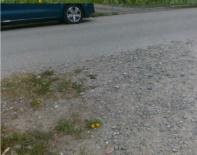
\includegraphics[height=30mm]{p6-000.png}};
    \node[right=8mm of a] (b) {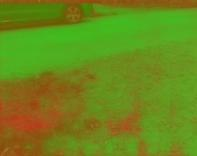
\includegraphics[height=30mm]{p6-001.png}};
    \node[right=8mm of b] (c) {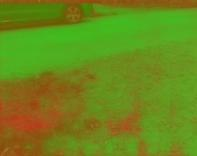
\includegraphics[height=30mm]{p6-001.png}};
    \node[font=\scriptsize, text=muted, above=1.2mm of a] {入力 RGB};
    \node[font=\scriptsize, text=muted, above=1.2mm of b] {コストマップ};
    \node[font=\scriptsize, text=muted, above=1.2mm of c] {ダイクストラの経路};
    \draw[kwarr] (a) -- (b);
    \draw[kwarr] (b) -- (c);
    \draw[cbluett, line width=0.9pt, -{Stealth[length=2mm]}]
      ([shift={(6mm,8mm)}]c.south west)
      to[out=75, in=210]
      ([shift={(-7mm,-8mm)}]c.north east);
    \node[font=\scriptsize, text=cbluett, anchor=east]
      at ([shift={(-2mm,1mm)}]c.north east) {経路};
  \end{tikzpicture}

  \takeaway{歩きやすさをコストにし，その上の最短経路を，歩く場所として使う．}
\end{frame}

\begin{frame}[plain]
  \vspace*{20mm}
  {\color{kickerblue}\footnotesize 次の系統\par}
  \vspace{4mm}
  {\fontsize{22}{26}\selectfont\bfseries\color{ink} Traversability-Aware\par}
  \vspace{3mm}
  {\color{ruleblue}\rule{\textwidth}{0.75pt}\par}
  \vspace{4mm}
  {\footnotesize\color{body}
    画像から歩きやすさを見積もり，コストマップの上で経路を決める．\par}
  \vspace{0pt plus 100fill}
  {\scriptsize\color{muted}\insertdate\hfill
    \insertframenumber/\inserttotalframenumber\par}
\end{frame}

\end{document}
